%----------------------GRUNDLAGEN --------------------

\chapter{Grundlagen}
\label{cha:grundlagen}
In diesem Kapitel werden die für die Studienarbeit relevanten Grundlagen betrachtet. Für die Abstandsmessung wird dabei das Ultraschallverfahren in \autoref {sec:ultraschall}erläutert. Als Antriebstechnik wird in \autoref{sec:schrittmotor} der Schrittmotor betrachtet und schließlich das \acrshort{mqtt}-Protokoll für die Kommunikation mit \autoref{sec:mqtt} beschrieben. 

\section{Abstandsmessung mit Ultraschall}
\label{sec:ultraschall}
Die Distanzmessung mit Ultraschall ist ein berührungsloses Verfahren. Die Messung  beruht auf dem Prinzip der Laufzeitmessung. Der Frequenzbereich von Ultraschall liegt zwischen 20Khz - 1Ghz (vgl. \cite{ultraschallbereich}) und somit außerhalb des hörbaren Bereichs (20Khz).  Das Frequenzspektrum bei technischen Anwendungen ist kleiner. \\
Ein Ultraschallsensor besteht aus einer Sende- und Empfangseinheit. Die Schallwellen werden meist auf Basis des piezoelektrischen Effekts impulsartig ausgesandt und ausgewertet.  Der Ultraschallimpuls pflanzt sich mit Schallgeschwindigkeit im Ausbreitungsmedium fort. Das zu messende Objekt reflektiert die Schallwelle. Die Empfangseinheit nimmt das entstandene Echo auf. Durch die verstrichene Zeit von der Aussendung bis zum Empfangen des Impulses kann die Entfernung des Objektes bestimmt werden. \\

Dabei gilt:
\begin{align}
d = \frac{1}{2} \cdot t\cdot c_U\\
\text{mit }  c_U \approx 340m/s 
\end{align}

\newpage
Die maximale Messdistanz hängt von der maximal möglichen Intensität der ausgesandter Wellen ab. Die minimale Messdistanz wird durch die Frequenz der Messung bestimmt (vgl. \cite{ultraschallUni}). \\
Prinzipbedingt unterliegen Ultraschallsensoren einigen Messfehlern. Dazu gehört, dass schallschluckende Oberflächen eine zu geringe Intensität reflektieren. Dasselbe gilt für Objekte mit rauer Oberfläche. Messfehler können außerdem durch sog. Scheinechos entstehen, wenn der Ultraschallimpuls von mehreren Objekten reflektiert wird. Aufgrund des Öffnungswinkels der Schalwelle ist der gleichzeitige Betrieb mehrerer Sensoren in derselben Richtung nur eingeschränkt möglich. (vgl. \cite{ultraschallBa})

\newpage
\section{Der Schrittmotor}
\label{sec:schrittmotor}
Der Schrittmotor zählt zu den \acrshort{synchronmaschine}n. Mit den Motoren können Positionen sehr exakt ohne weitere Regler angefahren werden. Schrittmotoren finden sich beispielsweise in Druckern, CD-Laufwerken und computergesteuerte Werkzeugmaschinen.  Schrittmotoren besitzen ein Haltemoment, das ebenfalls in vielen Anwendungen genutzt wird. (vgl. \cite{schrittmotorBa}, S. 2) In \autoref{pic:pmMotor} ist der Aufbau eines Schrittmotors \textit{(hier: PM-Motors)} dargestellt. 

\begin{figure}[h]
	\begin{center}
		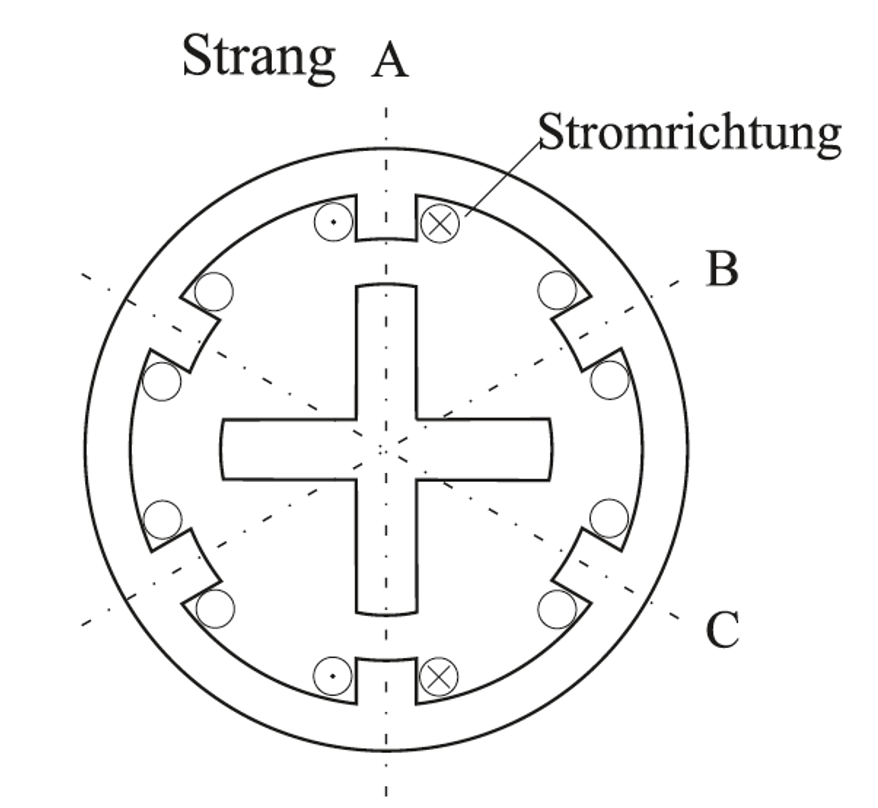
\includegraphics[width=7cm]{pmMotor.png}
		\caption{Prinzipieller Aufbau eines PM-Schrittmotors (\cite{kleinantriebe}, S.432)}
		\label{pic:pmMotor}
	\end{center}
\end{figure}


Prinzipiell folgt bei einem Schrittmotor ein Rotor dem sprungförmigen Weiterschalten des Statormagnetfeldes. Dadurch ergibt sich ein schrittweises Drehen um den Schrittwinkel $\alpha$. Nach Umschalten der Statorwicklung erfolgt die Drehung des Rotors nach einer kurzen Verzögerung. Nach einem Einschwingvorgang verharrt der Rotor für einen kurzen Moment in dieser Position. \newpage

 \autoref{pic:diagrammSchrittmotor} zeigt den zeitlichen Verlauf der mechanischen Winkelgeschwindigkeit  $\Omega_M$ und des Verdrehwinkels $\beta_M$ nach dem sprungförmigen Umschalten der Statorwicklung.  

 
\begin{figure}[h]
	\begin{center}
		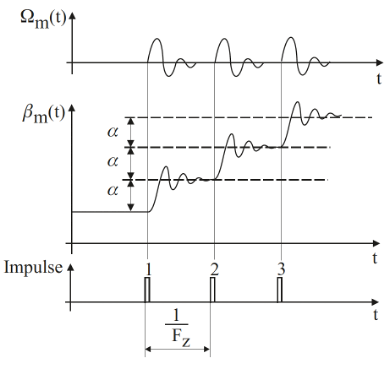
\includegraphics[width=9cm]{DiagrammVerlaufSchrittmotor.png}
		\caption{Zeitlicher Verlauf der mechanischen Winkelgeschwindigkeit $\Omega_m$ und des Verdrehwinkels $\beta_m$ in Folge elektrischer Impulse in den Statorwicklungen (hier: VR-Schrittmotor); \cite{kleinantriebe} S.433}
		\label{pic:diagrammSchrittmotor}
	\end{center}
\end{figure}



Da der Verdrehwinkel $\beta_M$ ein ganzzahliges Vielfaches des Schrittwinkels $\alpha$ ist, wird eine diskrete Positionierung ohne zusätzliche Sensorik möglich. Diese Art der Positionsbestimmung ist nur möglich, solange das maximale Drehmoment des Schrittmotors nicht überschritten wird. Ist das Lastmoment zu hoch, kommt es zu Schrittverlusten oder gar zum Stillstand.   Für die Ansteuerung eines Schrittmotors werden durch eine Steuerlogik Impulse erzeugt. Damit wird ein Leistungselektronik-Stellglied gesteuert, das die Statorwicklungen bestromt (vgl. \cite{kleinantriebe}, S. 432). \newline

Folgende Grundtypen von Schrittmotoren werden unterschieden: 
\begin{itemize}
	\item Reluktanz-Schrittmotor (VR)
	\item Permanenterregert Schrittmotor (PM)
	\item Hybrid-Schrittmotor (HY)
\end{itemize}

\newpage

\subsection{Der \acrshort{reluktanz}-Schrittmotor (VR)}

Beim \acrshort{reluktanz}-Schrittmotor besteht der Rotor aus einem Weicheisenkern dessen Zahnteilung ungleich der Polteilung des Stators ist. Nach einem Umschalten des Statormagnetfeldes bewegt sich der Rotor in die Position des geringsten magnetischen Widerstands (Reluktanz). Diese Stellung wird auch als \acrshort{koinzidenzstellung} bezeichnet. Die Stärke des magnetischen Feldes hängt von der Stromstärke ab. Diese ist veränderlich und verleiht dem Motortyp seine Bezeichnung VR-Motor \textit{(VR = engl. "variable reluctance motor")}. (vgl. \cite{schrittmotorBa}, S.2)

Für die Anzahl der Schritte je Umdrehung gilt: 

\begin{align}
	z = Z_R\cdot m_S 
\end{align}
\begin{center}
	mit $Z_R$ = Anzahl Rotorzähne und  $m_S$  = Strangzahl im Stator
\end{center}

Bei einem Motor mit vier Rotorzähnen und 3 Strängen würde sich somit bei einem Umschaltvorgang ein Verdrehwinkel $\beta$ von 30° einstellen. Um das Drehmoment zu erhöhen, werden alle Spulen gleichzeitig bestromt. Die Änderung des Magnetfeldes wird durch Umpolungen erreicht. 

\subsection{Der Permanenterregte Schrittmotor (PM)}
Beim PM-Motor ist der Rotor permanentmagnetisch. Dieser stellt sich ebenfalls in Abhänigigkeit vom Statormagnetfeld in polaritätsrichtige \acrshort{koinzidenzstellung}. Durch den Permanentmagneten bildet der Motor ein Haltemoment im stromlosen Zustand aus. Die Anzahl gleichzeitig erregter Wicklungen wird mit $n$ bezeichnet. Bei Verdopplung von $n$ halbiert sich der Schrittwinkel $\alpha$. Bleibt $n$ konstant, dreht sich der Rotor im \textit{Vollschrittbetrieb}. Bei einem PM-Motor kann zwischen Vollschritt- und Halbschrittbetrieb gewechselt werden. (vgl. \cite{kleinantriebe}, S. 436f). \newpage

\subsection{Der Hybrid-Schrittmotor (HY)}
Der Hybrid-Schrittmotor (HY) ist eine Kombination aus beiden Bauformen. Der Motor besitzt einen permanentmagnetischen Rotor sowie variabel ansteuerbare Statorwicklungen. Dadurch vereint die Bauform die Vorteile des hohen Drehmoments des PM-Motors sowie die große Auflösung des VR-Motors. Im Vergleich zum PM-Motor sind beim Hybrid-Schrittmotor Nord- und Südpol axial versetzt und um einen halben Zahn verdreht. Der Aufbau eines HY-Motors ist in \autoref{pic:hyMotor} dargestellt. 


\begin{figure}[h]
	\begin{center}
		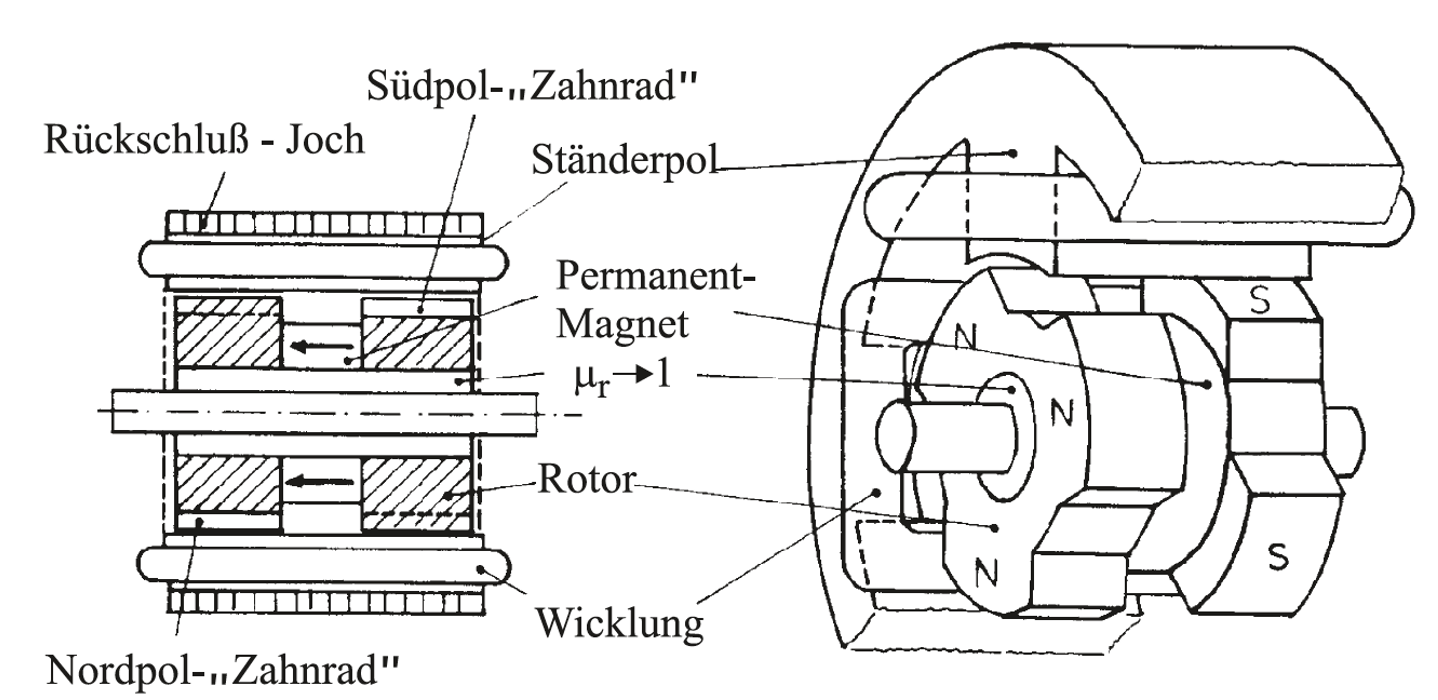
\includegraphics[width=10cm]{hyMotor.png}
		\caption{Aufbau eines Hybrid-Schrittmotors (HY) (\cite{kleinantriebe} S. 438)}
		\label{pic:hyMotor}
	\end{center}
\end{figure}

\newpage
Wie beim PM-Motor ermöglicht der HY-Motor ebenfalls den Betrieb im Vollschritt und Halbschritt. Im Vollschritbetrieb ist Anzahl bestromter Wicklungen $n$ konstant. Im Halbschrittbetrieb wechselt $n$. In \autoref{pic:schrittbetrieb} sind die Umschaltungsvorgänge der beiden Statorwicklungen dargestellt. 

\begin{figure}[h]
	\begin{center}
		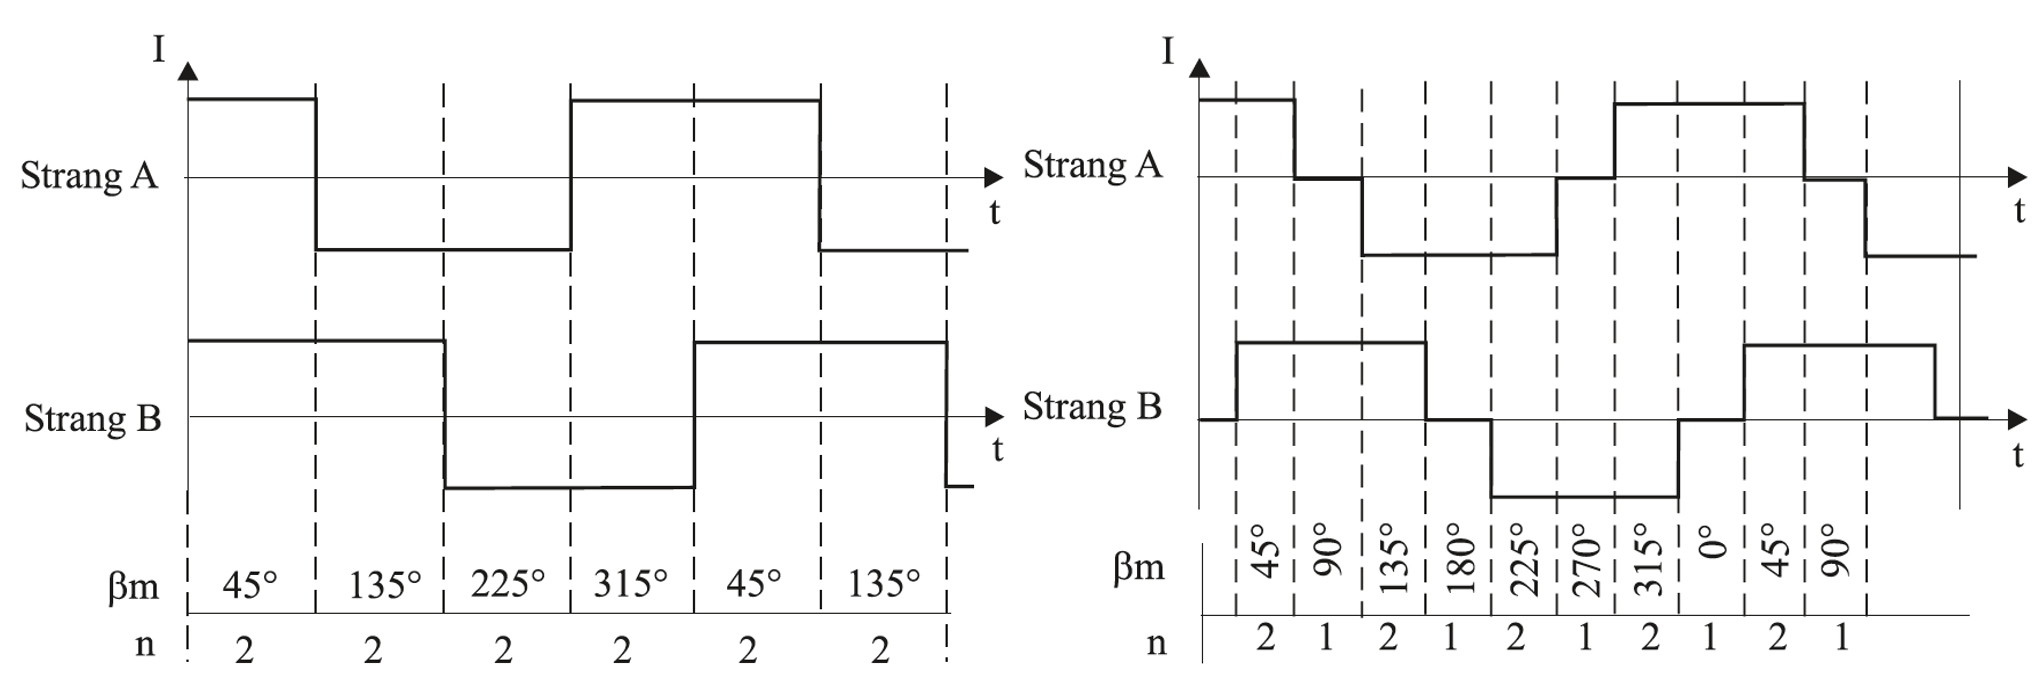
\includegraphics[width=16cm]{schrittbetrieb.png}
		\caption{Halbschritt- und Vollschrittbetrieb eines HY-Schrittmotors mit zwei Statorwicklungen (\cite{kleinantriebe} S. 454)}
		\label{pic:schrittbetrieb}
	\end{center}
\end{figure}


Wird $n$ größer, steigt dadurch Drehmoment $M$ des Motors. Durch die kontinuierliche Änderung von $n$ kann sich im Halbschrittbetrieb ein unrundes Laufverhalten ausprägen. \\
Eine weitere Betriebsart ist der Mikroschrittbetrieb. Dabei wird die Stromstärke in den Statorwicklungen durch den Treiber sinusförmig gesteuert. (vgl. \cite{kleinantriebe},S.438, 454; \cite{schrittmotorBa}, S.3)

\newpage
\section{MQTT} 
\label{sec:mqtt}
\acrfull{mqtt} ist ein Protokoll, welches zur digitalen Datenübertragung in ethernet-basierten Systemen dient. Es benötigt nur wenig Bandbreite und Ressourcen und verwendet eine 
Publish/Subscribe - Architektur. Das bedeutet, dass Nachrichten sogenannter Topics von Publishern bereitgestellt und von Subscribern empfangen werden. Der Datenverkehr wird über einen 
zentralen Broker verwaltet. In \autoref{pic:mqttbroker} ist eine typische \acrshort{mqtt}-Topologie aufgezeigt. 

\begin{figure}[h]
    \begin{center}
        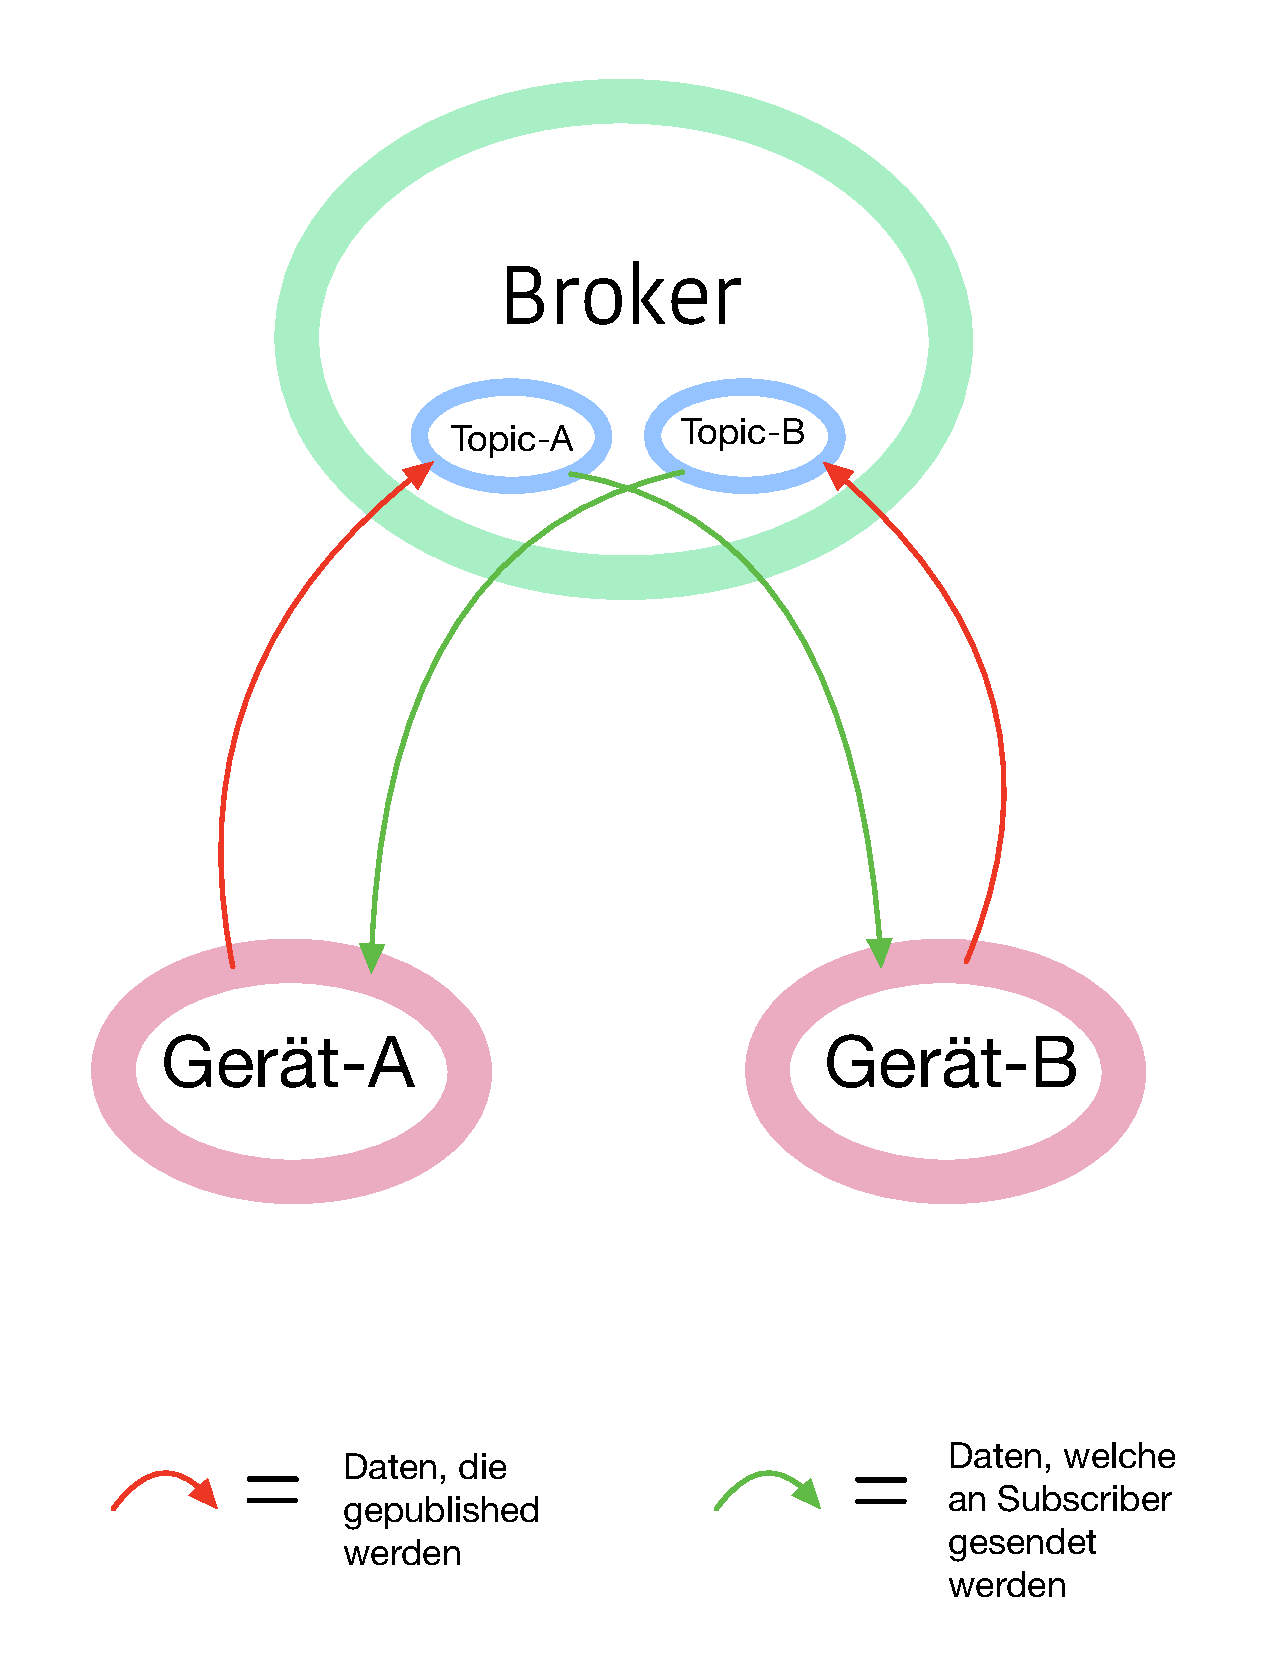
\includegraphics[width=11cm]{mqtt.pdf}
        \caption{
			\label{pic:mqttbroker}\acrshort{mqtt}-Datenübertragung über den Broker}
    \end{center}
\end{figure}

Zu sehen ist besagter Broker, welcher die Kommunikation verwaltet. Publisher schicken Daten an Topics, welche an Subscriber jener Topics übermittelt werden.
Um die Publish Subscribe Architektur zu verstehen, ist es hilfreich, die Analogie zum Fernsehen zu bilden. Dabei sendet ein TV-Sender sein Programm an einen bestimmten Kanal.
Auf diesen Kanal können nun beliebig viele Fernseher (Subscriber) zugreifen. Auch wenn keine aktive Verbindung zwischen Sender und Empfänger aufgebaut wird, erhalten beliebig viele Empfänger die benötigten Daten.
kennen, dass die Daten nicht zwischen Publisher und Subscriber direkt, sondern über den zentralen Broker versendet werden. \acrshort{mqtt} ist neben der einfachen Topologie auch für die sehr niedrige Netzlast bekannt. Echtzeitfähigkeit ist ebenfalls gegeben. (Vgl. \cite{mqtt})



\section{UART}
\label{sec:uart}
\acrfull{uart} bezeichnet eine Hardware-Schnittstelle, die zur seriellen Kommunikation zwischen zwei Geräten verwendet wird. In \autoref{pic:uartCon} ist die Verbindung zwischen zwei Geräten, die über \acrshort{uart} kommunizieren, gezeigt.

\begin{figure}[h]
    \begin{center}
        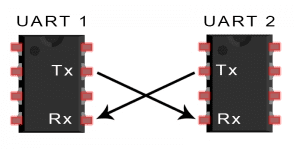
\includegraphics[width=8cm]{uart.PNG}
        \caption{\label{pic:uartCon}Verbindung zwischen zwei Geräten die über \acrshort{uart} kommunizieren}
    \end{center}
\end{figure}

Zu erkennen sind zwei Pins pro Gerät: Einer um Daten zu senden und einer um sie zu empfangen. Das generelle Prinzip von \acrshort{uart} ist, dass Daten in Pakete konvertiert werden, die dann Bit für Bit übermittelt werden. Ein Paket besteht aus einem Start-Bit, gefolgt von fünf bis neun Data-Bits, welche mit ein bis zwei Stop-Bits abgeschlossen werden. Daten werden also Byte für Byte an den Empfänger übertragen. Ein Arduino hat mehrere Pins, die für die \acrshort{uart}-Kommunikation verwendet werden können. In diesem Projekt werden nur die Standart-Pins verwendet, da nur zwei Geräte miteinander kommunikzieren müsen (vgl. \cite{uart}). 
\newpage
\section{Zustandsautomaten}
Ein Zustadsautomat ist ein Graph, bei dem die Knoten die Zustände des Automaten darstellen. Die Kanten zeigen die Übergangskriterien von einem in einen anderen Zustand (vgl. \cite{infoSkript}). In folgender Grafik ist ein einfacher Zustandsautomat aufgezeichnet: 

\begin{figure}[h]
	\begin{center}
		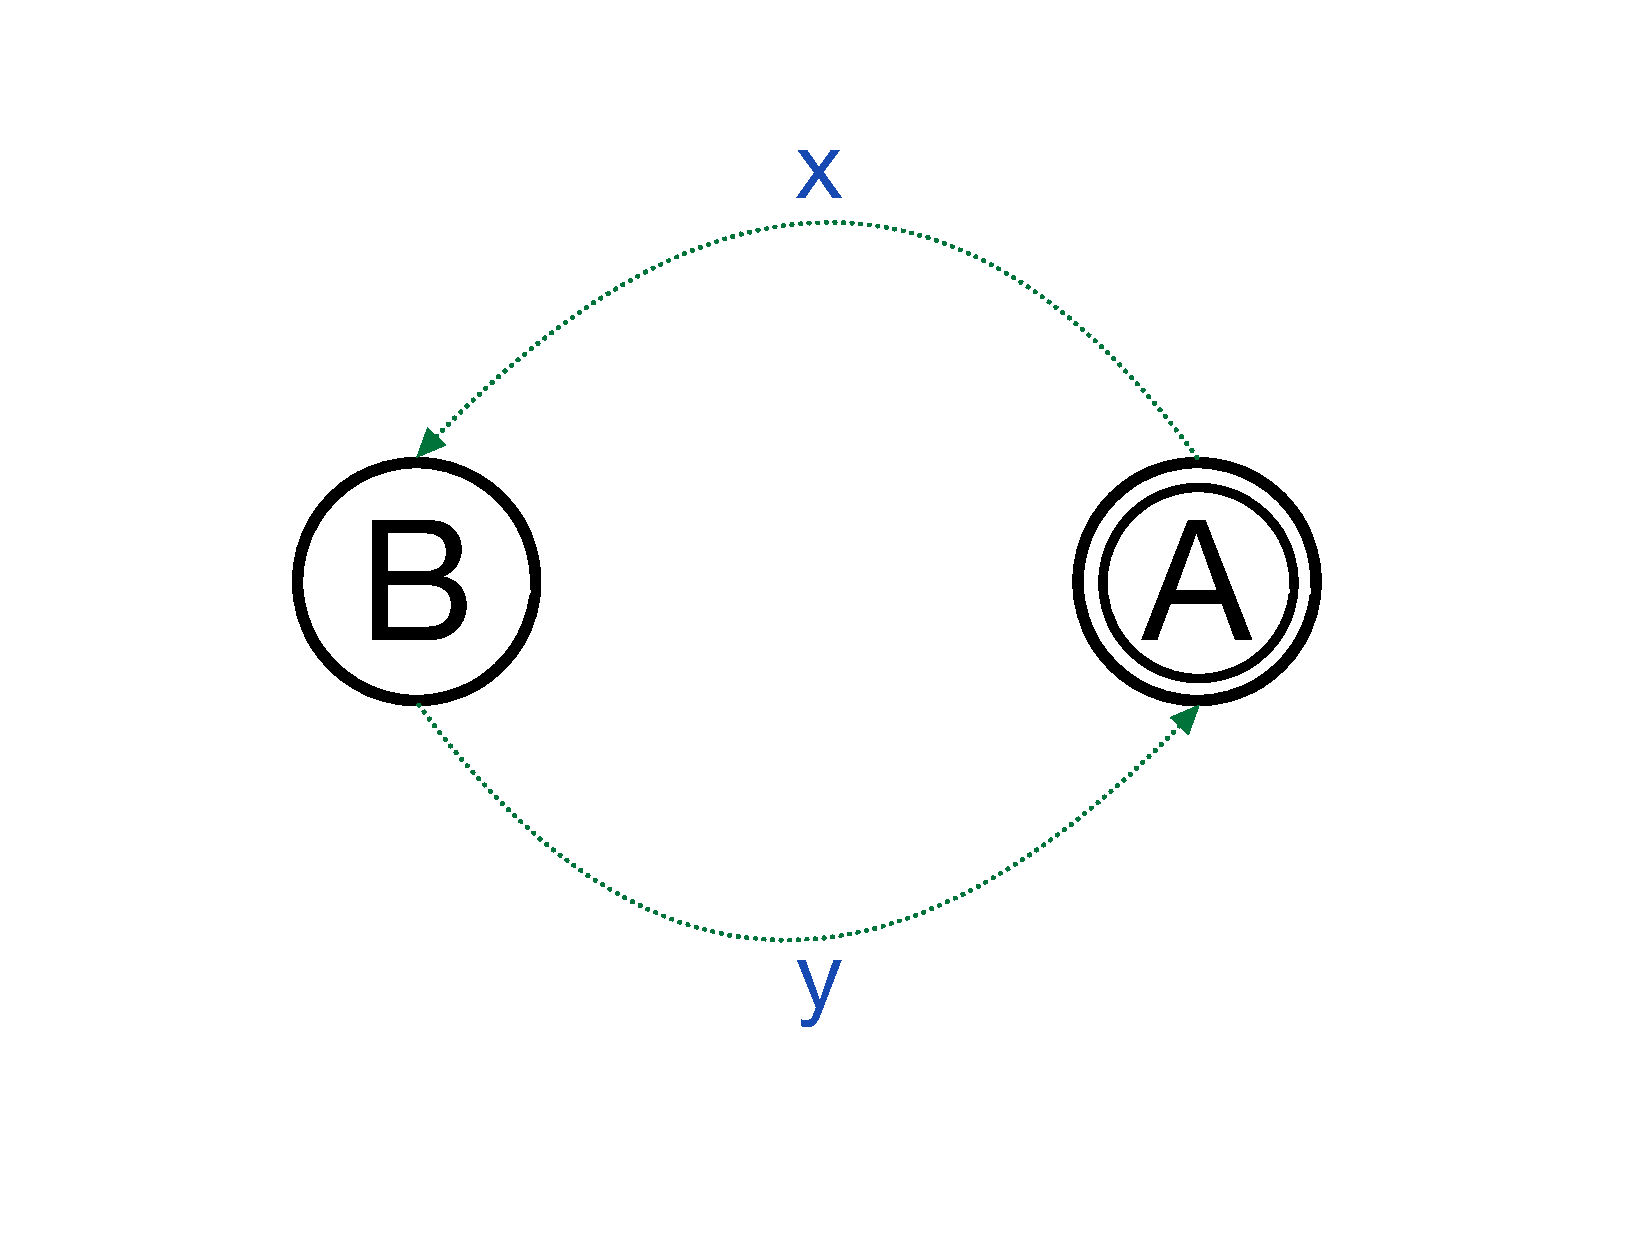
\includegraphics[width=9cm]{simpleState.pdf}
		\caption{\label{pic:simpleState}Einfacher Zustandsautomat}
	\end{center}
\end{figure}

In \autoref{pic:simpleState} ist ein Automat gezeigt, welcher zwei Zustände hat:$A$ und $B$. befindet er sich in Zustand $A$, kann er nur unter der Bedingung $x$ in Zustand $B$ wechseln und daraufhin auch nur über $y$ wieder zurück zu $A$. Die doppelte Umrandung von $A$ zeigt, dass es sich hierbei Um den Startzustand, also den zu beginnenden, Zustand handelt. \\
Zustandsautomaten finden oft Anwendung in Softwareentwicklung. Sie werden hauptsächlich verwendet um Nachrichten oder Eingaben zu lesen. In dieser Arbeit wird das GEsamtkonzept einzelner Softwarekomponenten als Zustandsautomaten implementiert.